\title{Lecture 5: Exponent and Logarithm}
\frame{\titlepage}


%%%%%%%%%%%%%
\section{Motivation}
\frame{\sectionpage}
%%%%%%%%%%%%%

\iffalse
\begin{frame}
\begin{figure}[h!]
\centering

\includegraphics[width = 0.7\textwidth]{l08i01.png}
\caption{Ultimate Werewolf Deluxe Edition}
\end{figure}
\end{frame}

\begin{frame}
\frametitle{Let's Play!}
\begin{center}
\Large Gangster of IDD
\end{center}
\begin{itemize}
\item 1 Criminal - Recruit one player (except the polices) to be part of the criminal gang at night \pa
\item 2 Polices - Know each other and immune to criminal recruit \pa
\item 1 Detective - Check the status of a player at night \pa
\item 1 Good citizen - Know the detective \pa
\item Citizen (the rest) - Help the polices and the detective find criminals. \pa
\end{itemize}
\end{frame}

\begin{frame}
\frametitle{Game Flow}
\begin{itemize}
\item Day - Everyone openly discusses who to catch. \pa If successful, the caught criminal is out of the game, and you may attempt to catch again. \pa If failed, the caught player is still in play.\pa
\item Night - Each criminal, individually, recruits one new team member.\pa
\end{itemize}
Win condition: \pa
\begin{itemize}
\item Criminal team wins if all but the polices are part of the criminal gang.  \pa
\item Police team (polices, detective, and citizens) wins if they catch all the criminals.
\end{itemize}
\end{frame}

\begin{frame}
\frametitle{Review}
\begin{figure}[h!]
\centering

\includegraphics[width = 0.5\textwidth]{l08i15.png}
\caption{YOU are the criminal! No, YOU!}
\end{figure}
\begin{itemize}
\item Before the play, which team did you think would win? Did they? \pa
\item Who has an easier time playing? Why? \pa
\item Is the game ``balanced''? 
\end{itemize}
\end{frame}
\fi

\begin{frame}
\frametitle{Level Up!}
\addfig{0.7}{l08i02}{Leveling system use exponential growth}{}
\end{frame}

\begin{frame}
\frametitle{Rapid Growth}
\addfig{0.7}{l08i03}{Rabbits, rabbits everywhere}
\end{frame}

\begin{frame}
\frametitle{Level Up (in a Scammy Way)}
\addfig{0.5}{l08i04}{\href{https://www.uspis.gov/news/scam-article/pyramid-schemes/}{MLM (Multi-level Marketing) a.k.a. pyramid scheme}}{}
\end{frame}

\begin{frame}
\frametitle{Compound Interest}
\addfig{0.7}{l08i05}{$M = (1 + a)^n$, $M$ = total money, $a$ = interest rate, $n$ = years}{}
\end{frame}

\begin{frame}
\addfig{0.3}{exponential_idle}{\href{https://www.youtube.com/watch?v=kMQ4PBjF0TI}{Exponential Idle (app)}}{}
\end{frame}

\begin{frame}
\frametitle{Test your exponential intuition 1} 
\begin{alertblock}{}
Assume a beautiful Lotus flower has a magical property to double every day. First day, there is only one lotus flower. Second day, there are 2 lotus flowers. Third day, there are 4 lotus flowers. 4th day there are 8 lotus flowers, then 16, then 32 and 64 and so on. 
\medskip

If it takes 30 days to fill the entire pond, and take over all the weeds, how many days does it take for the pond to be half full?
\end{alertblock}
\addfig{0.3}{expo_intuition_ex1}{Don't blink, or they will fill up your pond!}{}
\end{frame}

\begin{frame}
\frametitle{Test your exponential intuition 2} 
\begin{alertblock}{}
The inventor of chess requested his ruler give him wheat on the chessboard. He asked for 1 grain on the first space, 2 grains on the second space, 4 grains on the third space, 16 grains on the fourth space, and so on. The ruler laughs it off as a meager prize for a brilliant invention.
\medskip

How many grains of wheat are needed? (approximately)
\begin{tasks}(3)
\task $1,000,000$
\task $10^{20}$
\task $10^{30}$
\end{tasks}
\end{alertblock}
\addfig{0.2}{expo_intuition_ex2}{Don't ask me why they put rice grains on a chessboard....}{}
\end{frame}


%%%%%%%%%%%%%
\section[Exponential]{Exponential Function}
\frame{\sectionpage}
%%%%%%%%%%%%%

\begin{frame}
\frametitle{Choose one}
You are offered two boxes, $A$ and $B$, each with a label that has a function. \pa You have to choose one box, in which on day $x$, you will receive that amount of money.  Which box would you choose? \pa

\begin{remark}{}
\begin{eqnarray*}
A &\text{vs.}& B \\
10 \times x & \text{vs.}&  x^2 \\ \pa
10,000 \times x  & \text{vs.}& x^2 \\ \pa
10,000 \times x^2 & \text{vs.}& x^3 \\ \pa
x^2 & \text{vs.}& 2^x \\ \pa
x^{1,000,000} & \text{vs.}& 2^x \\ \pa
\end{eqnarray*}
\end{remark}
\end{frame}

\begin{frame}
\frametitle{Graph Comparison}
\begin{figure}[h!]
\centering

\includegraphics[width = 0.9\textwidth]{l08i06.png}
\end{figure}
\end{frame}

\begin{frame}
\frametitle{Basic definition}
Let $a$ be a positive integer and $M$ be a real number. Recall that we define the multiplication $a \times M$ to be
\[ a \times M = \underbrace{M + M + M + \cdots + M}_{a \text{ times}}\] \pa
\begin{defn}{}{}
Let $a$ be a positive integer and $M$ be a real number. We define the exponent $M^a$ (read $M$ to the power of $a$) to be
\[ M^a = \underbrace{M \times M \times M \times \cdots \times M}_{a \text{ times}}.\] 
\end{defn} \pa
\end{frame}


\begin{frame}[t]
\begin{ex}
Use the definition to compute the following numbers.
\begin{tasks}(4)
\task $3^2$
\task $5^3$
\task $2^{10}$
\task $7^1$
\end{tasks}
\end{ex}
\begin{sol}
\begin{tasks}(1)
\task $3^2 = 3 \times 3 = 9$
\task $5^3 = 5 \times 5 \times 5 = 125$
\task $2^{10} = 2 \times 2 \times 2 \times \cdots \times 2 = 1024$
\task $7^1 = 7$
\end{tasks}
\end{sol}
\end{frame}


\begin{frame}
\frametitle{Definition}
\begin{defn}{}{}
An \textbf{exponential function} is a function of the form 
\[ f(x) = a \times b^x\]
when $a$ is a positive real number.
\end{defn}

\begin{ex}
\[ 2^x, \quad 3 \times 10^x, \quad -  0.01^x, \quad \left( \frac{2}{25} \right)^x\]
\end{ex}
\end{frame}

\begin{frame}
\frametitle{Graph Comparison}
\begin{figure}[h!]
\centering

\includegraphics[width = 0.7\textwidth]{l08i08.png}
\end{figure}
\end{frame}

\begin{frame}[t]
\frametitle{Fraction Power}
What if $a$ is a rational number? Consider
\[M^{1/2}\]
\begin{slide}
Suppose that we have no idea how to define it yet. For this expression to make sense, it needs to agree with the definition. If we try to compute
\[M^{1/2} \times M^{1/2}\]
this would be as if we ``combine'' two halves to get a whole. Thus, we would expect
\[M^{1/2} \times M^{1/2} = M^1 = M\]
Actually, we already know that $\sqrt{M} \times \sqrt{M} = M$. Thus, it is natural to define
\[\sqrt{M} = M^{1/2}\]
\end{slide}
\end{frame}

\begin{frame}
\frametitle{Fractional Power}
\begin{defn}{}{}
For any integer $n$, define the $n$-th root of $M$ as
\[\sqrt[n]{M} = M^{1/n}\]
\tcblower

For any rational numberr $k= \frac{a}{b}$ be a rational number where $a,b$ are both integers and $b \neq 0$, define
\[ M^k = M^{a/b} = \sqrt[b]{M^a}\]
\end{defn}
\end{frame}

%%%%%%%%%%%%%
\section[Properties]{Properties of Exponential Function}
\frame{\sectionpage}
%%%%%%%%%%%%%

\begin{frame}[t]
\frametitle{How to Do Math}
Now that we have just defined a new operation, let's see if we can derive some basic properties based on the definition.
\begin{block}{}
\[ M^{a+b}\]
\end{block}
\begin{slide}
\begin{eqnarray*}
M^{a+b} &=& \underbrace{M \times M \times \cdots \times M}_{a+b \text{ times}} \\ \pa
&=& \underbrace{M \times M \times \cdots \times M}_{a \text{ times}} \times \underbrace{M \times M \times \cdots \times M}_{b \text{ times}} \\ \pa
&=& M^a \times M^b
\end{eqnarray*}
Thus, we conclude that
\[M^{a+b} = M^a \times M^b.\]
\end{slide}
\end{frame}



\begin{frame}[t]
\begin{block}{}
\[(M \times N)^a\]
\end{block}
\begin{slide}
We treat $M \times N$ as a single number and apply the definition.
\begin{eqnarray*}
(M \times N)^a &=& \underbrace{(M \times N) \times (M \times N) \times \cdots \times (M \times N)}_{a \text{ times}} \\ \pa
&=& \underbrace{M \times M \times \cdots \times M}_{a \text{ times}} \times \underbrace{N \times N \times \cdots \times N}_{a \text{ times}} \\ \pa
&=& M^a \times N^a
\end{eqnarray*}
Thus, we conclude that
\[(M \times N)^a = M^a \times N^a.\]
\end{slide}
\end{frame}


\begin{frame}[t]
\begin{block}{}
\[(M^a)^b\]
\end{block}
\begin{slide}
We treat $M^a$ as a single number and apply the definition.
\begin{eqnarray*}
(M^a)^b &=&  \underbrace{M^a \times M^a \times \cdots \times M^a}_{b \text{ times}} \\ \pa
&=& M^{(\overbrace{a+a+\cdots+a}^{b \text{ times}})} \\ \pa
&=& M^{a\times b}
\end{eqnarray*}
Thus, we conclude that
\[(M^a)^b = M^{a \times b}.\]
\end{slide}
\end{frame}


\begin{frame}[t]
\begin{block}{}
\[M^0\]
\end{block}
\begin{slide}
If we apply the first property with $b=0$ we have
\begin{eq*}
M^{a+0} &=& M^a \times M^0 \\
M^a &=& M^a \times M^0 
\end{eq*}
For the equation to hold, we need
\[M^0 = 1.\]
\medskip

Alternately, we notice that if going up (say from $M^3$ to $M^4$) means we multiply by $M$, then going down (say from $M^2$ to $M^1$) means dividing by $M$. This means
\[\frac{M^3}{M^2} = M, \quad \frac{M^2}{M^1} = M, \quad \frac{M^1}{M^0} = M, \quad \then M^0 = 1\]
\end{slide}
\end{frame}

\begin{frame}[t]
\begin{block}{}
\[M^{-a}\]
\end{block}
\begin{slide}
We know that 
\[M^a \times M^{-a} = M^{a + (-a)} = M^0 = 1.\] \pa
And also, 
\[M^a \times \frac{1}{M^a} = \frac{M^a}{M^a} = 1.\] \pa
Thus, we conclude that
\[M^{-a} = \frac{1}{M^a}.\]
Since we can multiply $M^a$ by $M^{-a}$ to get 1, we call $M^{-a}$ the \textbf{multiplicative inverse} of $M^a$.
\end{slide}
\end{frame}

\begin{frame}
\frametitle{Properties}
We summarize the properties as follows.
\begin{prop}{}{}
Let $M,N$ be positive real numbers, and $a,b$ be real numbers. \pa
\begin{enumerate}
\item $M^{a+b} = M^a \times M^b$ \pa
\item $(M\times N)^a = M^a \times N^a$ \pa
\item $(M^a)^b = M^{a \times b}$ \pa
\item $M^0 = 1$ \pa
\item $\displaystyle M^{-a} = \frac{1}{M^a}$ \pa
\end{enumerate}
\end{prop}
\end{frame}

\begin{frame}
\frametitle{Caution}
\begin{slide}
Note:
\begin{itemize} 
\item If $M \neq N$ and $a \neq b$, then $M^a \times N^b$ cannot be combined (for instance, $2^5 \times 3^{0.7}$ should be left as is). \pa
\item A common mistake is to use exponent property with addition
\begin{alertblock}{}
\[ (a+b)^2 \neq a^2 + b^2 \]
\end{alertblock}
The correct approach is to transform the exponent into simple multiplication.
\begin{eq*}
(a+b)^2 &=& (a+b) \times (a+b) \\
&=& a \times (a+b) + b \times (a+b) \mathnote{distributive} \\
&=& (a \times a) + (a \times b) + (b \times a) + (b \times b) \\
&=& a^2 + 2ab + b^2
\end{eq*}
\end{itemize}
\end{slide}
\end{frame}


\begin{frame}[t]
\begin{ex}
Simplify the following terms using properties.
\begin{tasks}(4)
\task $3^4 \times 3^5$
\task $2^{-2} \times 2^{3}$
\task $2^7 \times 3^7$
\task $9^3 \times 2^6$
\end{tasks}
\end{ex}
\begin{sol}
\begin{tasks}(1)
\task $3^4 \times 3^5 = (3 \times 3 \times 3 \times 3) \times (3 \times 3 \times 3 \times 3 \times 3) = 3^9$
\task $2^{-2} \times 2^{3} = \frac{1}{2 \times 2} \times (2 \times 2 \times 2) = 2$
\task $2^7 \times 3^7 = \underbrace{(2 \times 2 \times \cdots \times 2)}_{7 \text{ times}} \times \underbrace{(3 \times 3 \times \times \cdots 3)}_{7 \text{ times}} = (2 \times 3) \times (2 \times 3) \times \cdots \times (2 \times 3) = (2 \times 3)^7 = 6^7$
\task Neither the bases of the exponents are the same. Nevertheless, we can convert the exponents to match. $9^3 \times 5^6 = (3^2)^3 \times 5^6 = 3^{(2 \times 3)} \times 5^6 = 3^6 \times 5^6 = (15)^6$
\end{tasks}
\end{sol}
\end{frame}

\begin{frame}
\begin{exercisebox}{}{}
Use the properties to simplify the following terms. \textbf{Do not} blindly apply the formulas.
\begin{enumerate}
\item $2^3 \times 2^4$
\item $3^5 \times 3^{-7}$
\item $2^8 \times 3^8$
\item $4^{-3} \times 5^{-3}$
\item $5^{10} \times 4^{5}$
\item $(2^4)^5$
\end{enumerate}
\end{exercisebox}
\end{frame}



%%%%%%%%%%%%%
\section[Application]{Application of Exponential}
\frame{\sectionpage}
%%%%%%%%%%%%%

\begin{frame}[t]
\frametitle{Population Growth}
\begin{thm}{}{}
A growth (or decay) can be modeled by the function
\[ f(t) = a (1+b)^t, \]
where $t$ represents time, and $a$ and $b$ are some constant with $b>0$.
\begin{itemize}
\item If $b>0$, we call $f$ a growth function.
\item If $-1<b,0$, we call $f$ a decay function.
\end{itemize}
\end{thm}
\end{frame}

\begin{frame}[t]
\begin{ex}
Suppose that the population of India was about 1.25 billion in the year 2013, with an annual growth rate of about 1.2\%. What will the population of India be in 2031?
\end{ex}
\begin{sol}
This situation can be represented by the growth function
\[ f(t) = 1.25 (1 + 12\%)^t = 1.25(1.012)^t, \]
where $t$ is a number of years (since 2013). Notice that at the start when $t=0$, we have $f(t) = 1.25 (1.012)^0 = 1.25$ as intended.

Now, from 2013 to 2031, it'll take $2031-2013 = 18$ years, and so we can plug in $t=18$ into the function to get 
\[ f(18) = 1.25 (1.012)^{18} \approx 1.549.\]

Thus, the population of India in 2031 would be about 1.549 billion.
\end{sol}
\end{frame}

\begin{frame}[t]
\begin{ex}
A scientist begins with 100 milligrams of a radioactive substance that decays exponentially. After 35 hours, 50mg of the substance remains. How many milligrams will remain after 54 hours?
\end{ex}
\begin{sol}
This situation can be represented by a decay function
\[ f(t) = a (1 + b)^t =100(1+b)^t,\]
where $b$ is some constant. We know that 
\begin{eq*}
f(35) &=& 50 = 100(1+b)^{35} \\
(1+b)^{35} &=& \tfrac{1}{2} \\
1+b &=& \left(\tfrac{1}{2}\right)^{1/35}
\end{eq*}
Hence, we can compute the amount of substance when $t=54$ to be
\[ f(54) = 100\left( \tfrac{1}{2^{1/35}}\right)^{54} \approx 34.321\]
\end{sol}
\end{frame}

\begin{frame}[t]
\frametitle{Compound Interest}
\begin{thm}{}{}
Let 
\begin{itemize}
\item $P$ be the principal,
\item $r$ be the annual percentage rate (APR),
\item $n$ be the number of compouding periods in a year,
\item $t$ be the time.
\end{itemize}
Then the account value by the end of time $t$ is
\[ A(t) = P\left(1+ \frac{r}{n}\right)^{nt}.\]
\end{thm}
\end{frame}

\begin{frame}[t]
\begin{ex}
If we invest \$3,000 in an investment account paying 3\% interest compounded quarterly, how much will the account be worth in 10 years?
\end{ex}
\begin{sol}
We are starting with $P=3000$. Our interest rate is 3\%, so  $r=0.03$. Because we are compounding quarterly, we are compounding 4 times per year, so  $n=4$. We want to know the value of the account in 10 years, so we are looking for $A(10)$. Thus, we have
\begin{eq*}
A(t) &=& P\left(1+\frac{r}{n}\right)^{nt} \\
A(10) &=& 3000 \left(1+\frac{0.03}{4}\right)^{4 \times 10} \\
&\approx& 4045.05
\end{eq*}
\end{sol}
\end{frame}

\begin{frame}
\begin{exercisebox}{}{}
\begin{enumerate}
\item The fox population in a certain region has an annual growth rate of 9\% per year. In the year 2012, there were 23,900 fox counted in the area. What is the fox population predicted to be in the year 2020?
\item A car was valued at \$38,000 in the year 2007. By 2013, the value had depreciated to \$11,000. If the car’s value continues to drop by the same percentage, what will it be worth by 2017?
\item If we opended an investment account with an initial deposit of \$4,000 and with an annual interest rate of 7\%, compounding quarterly, how much will the account be worth in 9 years? 
\end{enumerate}
\end{exercisebox}
\end{frame}

%%%%%%%%%%%%%
\section{Logarithm}
\frame{\sectionpage}
%%%%%%%%%%%%%

\begin{frame}[t]
\frametitle{Inverse Problem}
Recall the Wheat and Chessboard problem. 
\begin{slide}
We know that on $k$-th space, there will be $2^k$ grains of wheat. At some point, we will run out of grains of wheat to put on the board. Suppose you have one million grains. You will be interested in asking the following question:

\begin{question}{}
What is the first space does the number of grains of wheat exceeds one million?
\end{question}
To find the solution, we want to solve for
\[2^k \geq 1000000\]
and want a solution in the form
\[k \geq ?\]
\end{slide}
\end{frame}


\begin{frame}
\frametitle{Definition}
We can't achieve this via addition nor multiplication, so we will need to define a new function.
\begin{defn}{}{}
Let $x > 0$ and $b > 0$ with $b \neq 1$. Then, if we have
\[x = b^y\]
then, we define the logarithm as
\[ \log_b x = y.\]
In other words, $\log_b x$ is asking: $b$ to the what equals $x$?

We read this logarithmic expression as ``The logarithm with base $b$ of $x$ equals $y$.
\end{defn} \pa
\end{frame}

\begin{frame}
\begin{figure}[h!]
\centering
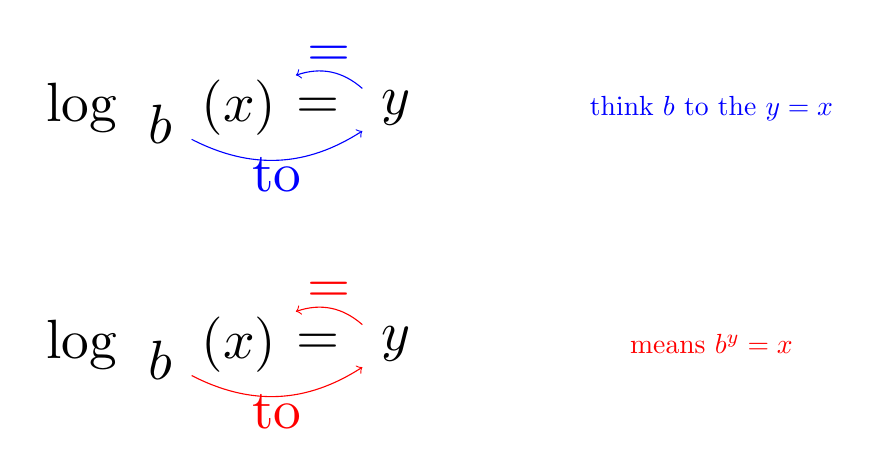
\begin{tikzpicture}[every node/.style={scale = 2}]
\node at (0,0) {log};
\node at (2,0) (X) {$(x)$};
\node at (3,0) {$=$};
\node at (4,0) (Y) {$y$};
\node at (1,-0.2) (B) {$b$};
\draw[->, blue] (B) to[bend right] (Y);
\draw[opacity = 0] (B) -- (Y) node [pos=0.5, below = 4pt, blue, opacity = 1] {to};
\draw[->, blue ] (Y) to[bend right] (X);
\draw[opacity = 0 ] (Y) -- (X) node [pos =0.5, above = 4pt, blue, opacity = 1] {$=$};
\node at (8,0) [scale = 0.5, blue] {think $b$ to the $y = x$};

\begin{scope}[yshift = -3cm]
\node at (0,0) {log};
\node at (2,0) (X) {$(x)$};
\node at (3,0) {$=$};
\node at (4,0) (Y) {$y$};
\node at (1,-0.2) (B) {$b$};
\draw[->, red] (B) to[bend right] (Y);
\draw[opacity = 0] (B) -- (Y) node [pos=0.5, below = 4pt, red, opacity = 1] {to};
\draw[->, red] (Y) to[bend right] (X);
\draw[opacity = 0 ] (Y) -- (X) node [pos =0.5, above = 4pt, red, opacity = 1] {$=$};
\node at (8,0) [scale = 0.5, red] {means $b^y=x$};
\end{scope}
\end{tikzpicture}
\caption{Illustration for the notation of logarithm.}
\end{figure}
\end{frame}

\begin{frame}[t]
\begin{ex}
Convert each exponential equation into a logarithm equation.
\begin{tasks}(3)
\task $2^{6} = 64$
\task $3^{4} = 81$
\task $4^{-2} = \frac{1}{16}$
\end{tasks}
\end{ex}
\begin{sol}
\begin{tasks}(1)
\task $\log_2 64 = 6$
\task $\log_3 81 = 4$
\task $\log_4 \frac{1}{16} = -2$
\end{tasks}
\end{sol}
\end{frame}


\begin{frame}[t]
\begin{ex}
Use definition of logarithm function to find the following.
\begin{tasks}(3)
\task $\log_3 9$ 
\task $\log_4 64$ 
\task $\log_2 \frac{1}{32}$
\end{tasks}
\end{ex}
\begin{sol}
\begin{tasks}(1)
\task $\log_3 9$ is the number $x$ such that $3^x = 9$, so $\log_3 9 = x = 2.$ \pa
\task $\log_4 64$ is the number $x$ such that $4^x = 64$ so $\log_4 64 = x = 3.$ \pa
\task $\log_2 \frac{1}{32}$ is the number $x$ such that $2^x = \frac{1}{32} = 2^{-5}$ so $\log_2 \frac{1}{32} = x = -5$.
\end{tasks}
\end{sol}
\end{frame}

\begin{frame}
\frametitle{Graph Comparison}
\begin{figure}[h!]
\centering

\includegraphics[width = 0.9\textwidth]{l08i10.png}
\end{figure}
\end{frame}

\begin{frame}
\frametitle{Note on definition}
\begin{question}{}
Is it necessary that $b > 0$? Why can't we have $b=1$?
\tcbsubtitle{Answer}
Yes. Because $f(x) = \log_{-2} x$ is not a function. There is no solution for some value of $x$. For instance, $(-2)^y = 8$ has no solution. 
\medskip

To avoid the issue, we require the base $b$ to be positive. Then, the function would be defined for all positive real numbers $x$.

Similarly, if $b=1$, then the equation becomes $1^y = x$, but $1^y = 1$ for all real numbers $y$, so we don't get a function either.
\end{question}
\end{frame}

\begin{frame}
\frametitle{Note on definition}
\begin{question}{}
Is it necessary that $x > 0$?
\tcbsubtitle{Answer}
Yes. Once we require the base $b$ to be positive, an expression like $\log_b (-5)$ has no solution. It is impossible to find a real number $y$ such that $b^y = -5$.
\end{question}
\end{frame}



%%%%%%%%%%%%%
\section[Properties]{Properties of Logarithm Function}
\frame{\sectionpage}
%%%%%%%%%%%%%

\begin{frame}[t]
\frametitle{Deriving Properties}
All properties of logarithm function can be derived from exponential function. For instance, we have
\begin{block}{}
\[M^0 = 1,\]
\end{block}
\begin{slide}
so we then have
\[\log_M 1 = 0.\]

Likewise, from
\begin{block}{}
\[M^{-a} = \frac{1}{M^a}\]
\end{block}
we can derive
\[\log_M \frac{1}{M^a} = -a\]
\end{slide}
\end{frame}

\begin{frame}[t]
\frametitle{}
Another example is
\begin{block}{}
\[M^a \times M^b = M^{a+b}\]
\end{block}
\begin{slide}
If we take logarithm on both sides, we get
\[\log_M (M^a \times M^b) = \log_M (M^{a+b}) = a+b.\]
Then, if we let 
\[A = M^a \text{ and } B = M^b,\]
then by definition we have
\[\log_M A = a \text{ and } \log_M B = b.\]
 When we replace $M^a$ and $M^b$ on the left-handed side, and $a+b$ on the right-handed side by the logarithms we just derived, we have
 \[\log_M (A \times B) = \log_M A + \log_M B\]
\end{slide}
\end{frame}

\begin{frame}[t]
\frametitle{}
Division works similarly. If we replace $b$ by $-b$, we get
\begin{block}{}
\[M^a \times M^{-b} = M^{a-b}\]
\end{block}
\begin{slide}
We can rewrite $M^{-b} = \frac{1}{M^b}$ to get
\[\frac{M^a}{M^b} = M^{a-b}.\]
Thus, we have
\[\log_M \left( \frac{A}{B} \right) = \log_M A - \log_M B\]
\end{slide}
\end{frame}

\begin{frame}[t]
\frametitle{}
If we apply the property
 \[\log_M (A \times B) = \log_M A + \log_M B\]
where $A=B$, we have
\begin{slide}
\[\log_M (A^2) = \log_M A + \log_M A = 2 \log_M A\]
We can continue multiplying by the same value to get
\[\log_M (A^3) = \log_M A + \log_M A + \log_M A = 3 \log_M A.\]
In general, if $n$ is a natural number, we have
\begin{eq*}
\log_M (A^n) &=& \underbrace{\log_M A + \log_M A + \cdots + \log_M A}_{n \text{ times}} \\
&=&n \log_M A
\end{eq*}
Furthermore, we can expand this definition to work not only for integers, but also for all real numbers!
\end{slide}
\end{frame}

\begin{frame}[t]
\frametitle{}
The remaining property is
\begin{block}{}
\[(M^a)^b = M^{ab}\]
\end{block}
\begin{slide}
We then have
\[\log_M (M^a)^b = \log_M M^{ab} = ab\]
If we let $A = M^a$ and $B = (M^a)^b = A^b$, we then have $\log_M A = a$ and $\log_A B = b$ and so
\[\log_M B = \log_M A \log_A B\]
This form is a chain property. We can rewrite so that logarithms base $M$ are on the same side.
\[\frac{\log_M B}{\log_M A} = \log_A B\]
This is useful when you want to change from one base to another.
\end{slide}
\end{frame}

\begin{frame}
\begin{prop}{}{}
Let $M,N, a$ be positive real numbers. \pa
\begin{enumerate}
\item $\log_a 1 = 0$
\item $\log_a (M \times N) = \log_a M + \log_a N$ \pa
\item $\log_a \left( \frac{M}{N}\right) = \log_a M - \log_a N$ \pa
\item $\log_a (M^b) = b \times \log_a M$, for any real number $b$ \pa
\item $ \log_a M = \frac{\log_b M}{\log_b a}$, for any positive real number $b$ \pa
\end{enumerate}
\end{prop}
\end{frame}


\begin{frame}[t]
\begin{ex}
Use the properties to simplify the following terms
\begin{tasks}(2)
\task $\log_2 8 + \log_2 32$
\task $\log_3 36 - \log_3 4$
\task $\frac{\log_5 81}{\log_5 3}$
\task $\log_5 \left(\frac{1}{2^4} \right)$ 
\end{tasks}
\end{ex}
\begin{sol}
\begin{tasks}(1)
\task $\log_2 8 + \log_2 32 = \log_2 (8 \times 32) = \log_2 (256) = 7$
\task $\log_3 36 - \log_3 4 = \log_3 \left( \frac{36}{4} \right) = \log_3 (9) = 2$
\task $\frac{\log_5 81}{\log_5 3} = \log_{3} (81) = 4$
\task $\log_5 \left(\frac{1}{2^4} \right) = \log_5 \left( \frac{1}{2} \right)^4 = \log_5 (2^{-4}) = -4 \log_5 2$  
\end{tasks}
\end{sol}
\end{frame}

\begin{frame}
\frametitle{Conventions}
\begin{defn}{}{}
If $\log$ is written without the base, we assume that it is in base 10*. In other words,
\[\log x = \log_{10} x\]
\end{defn}

\begin{defn}{}{}
As $\log$ base $e, \quad (e \approx 2.718)$ is frequently used, we define it as
\[\ln x = \log_e x \]
It reads ``the natural log of $x$'' or ``lon''.
\end{defn}
{\small *unless you are a computer scientist who uses base 2}
\end{frame}

\begin{frame}
\begin{exercisebox}{}{}
Use the properties to simplify the following terms
\begin{enumerate}
\item $\log_6 4 + \log_6 9$
\item $\log_2 20 - \log_2 5$
\item $\frac{\log_3 16}{\log_3 2}$
\item $\log_2 (5^{-8})$ 
\end{enumerate}
\end{exercisebox}
\end{frame}


%%%%%%%%%%%%%
\section[Application]{Application of Logarithm}
\frame{\sectionpage}
%%%%%%%%%%%%%

\begin{frame}
\frametitle{Logarithm in Science}
\begin{figure}[h!]
\centering

\includegraphics[width = 0.8\textwidth]{l08i12.png}
\caption{Decibel}
\end{figure}
\end{frame}

\begin{frame}
\frametitle{Logarithm in Science}
\begin{figure}[h!]

\includegraphics[width = 0.7\textwidth]{l08i13.png}
\caption{pH}
\end{figure}
\end{frame}

\begin{frame}
\frametitle{Logarithm in Science}
Earthquake (Richter magnitude)
\begin{figure}[h!]
\centering

\includegraphics[width=0.3\linewidth]{l08i11.png} 
\end{figure}
\end{frame}

\begin{frame}[t]
\frametitle{Number of Digits}
\begin{question}{}
How many digits does $2^{100}$ have?
\end{question} 
\begin{slide}
It may seem intimidating for such a large number, so we first find some pattern for smaller numbers.
\begin{itemize}
\item Integers between 0 and 9 have 1 digit.
\item Integers between 10 and 99 have 2 digits.
\item Integers between 100 and 999 have 3 digits.
\item Integers between 1000 and 9999 have 4 digits.
\item $\vdots$
\item Integers between $10^k$ and $10^{k+1} - 1$ have $k+1$ digits.
\end{itemize}
\end{slide}
\end{frame}

\begin{frame}[t]
\frametitle{Pattern}
Then, how can we simply such numbers? We use the fact that logarithm function is increasing and apply to the inequalities. If $x$ has $k$ digits, then we have
\begin{slide}
\begin{eq*}
10^{k-1} &\leq& x \quad < 10^{k} \\
\log_{10} 10^{k-1} &\leq& \log_{10} x < \log_{10} (10^{k}) \\
k-1 &\leq& \log_{10} x < k
\end{eq*}
We can summarize this observation (which is almost a proof) as follows.
\end{slide}
\end{frame}

\begin{frame}
\frametitle{Logarithm in Math}
\begin{thm}{}{}
Let $N$ be a real number. Then, the number of digits of $N$ in base 10 is
\[ \lfloor \log_{10} N \rfloor + 1,\]
where $\lfloor x \rfloor$ (called the floor function) is rounding $x$ down to the closest integer.

\tcblower

In general, the number of digits $N$ in base $k$ is
\[ \lfloor \log_{k} N \rfloor + 1.\]
\end{thm}
\end{frame}


\begin{frame}[t]
\begin{ex}
How many digits does $2^{100}$ have in base 10? Use the approximation $\log_{10} 2 \approx 0.3010.$
\end{ex}
\begin{sol}
The number of digits is
\begin{eq*}
\lfloor \log_{10} 2^{100} \rfloor + 1 &=& \lfloor 100 \times \log_{10} 2 \rfloor + 1 \\
&\approx& \lfloor 100 \times (0.3010) \rfloor + 1 \\
&=& \lfloor 30.10 \rfloor + 1 \\
&=& 30 + 1 = 31
\end{eq*}
Thus, $2^{100}$ has 31 digits. A calculator would give you $1.267 \times 10^{30}$, which means it has the leading digit of 1 followed by 30 digits, for the total of 31 digits.
\end{sol}
\end{frame}


\begin{frame}[t]
\begin{ex}
How many digits does $10^{100}$ have in base 2? Use the approximation $\log_{10} 2 \approx 0.3010.$
\end{ex}
\begin{sol}
First of all, we can use the property of logarithm function to find 
$\log_{2} 10 = \frac{1}{\log_{10} 2} \approx \frac{1}{0.3010} \approx 3.3226.$ 
Now we can compute the number of digits in base 2 to be
\begin{eq*}
\lfloor \log_{2} 10^{100} \rfloor + 1 &=& \lfloor 100 \times \log_{2} 10 \rfloor + 1 \\
&\approx& \lfloor 332.226 \rfloor + 1 \\
&=& \lfloor 332.226 \rfloor + 1 \\
&=& 332 + 1 = 333
\end{eq*}
Thus, $10^{100}$ has 333 digits in base 2.
\end{sol}
\end{frame}


\begin{frame}[t]
\begin{ex}
A standard deck of cards consists of 52 cards. It is known that it is unlikely that two well-shuffled deck of cards would have the same arrangements. 
\medskip

It is know that the number of different arrangements is $52!$, where $!$ is the factorial. How many digits does $52!$ have in base 10?
\end{ex}
\begin{sol}
First, we simplify $\log_{10} 52!$ using the multiplication property:
\begin{eq*}
\log_{10} 52! &=& \log_{10} (52 \times 51 \times 50 \times \cdots \times 3 \times 2 \times 1) \\
&=& \log_{10} 52 + \log_{10} 51 + \cdots + \log_{10} 3 + \log_{10} 2 + \log_{10} 1 \\
&\approx& 1.716 + 1.707 + \cdots + 0.477 + 0.301 + 0 \\
&\approx& 67.906
\end{eq*}
Thus, the number of digits is
\[\lfloor \log_{10} 52! \rfloor + 1 = \lfloor 67.906 \rfloor + 1 = 68.\]
\end{sol}
\end{frame}

\begin{frame}
\begin{exercisebox}{}{}
For the following problems, use these approximations
\[\log_{10} 2 \approx 0.301, \quad \log_{10} 3 \approx 0.477, \quad \log_5 10 \approx 1.4306\]
\begin{enumerate}
\item How many digits does $3^{100}$ have in base 10?
\item How many digits does $10^{100}$ have in base 5?
\item Which number is larger: $2^{100}$ or $3^{60}$? Prove by counting the number of digits for each number.
\end{enumerate}
\end{exercisebox}
\end{frame}

%%%%%%%%%%%%%
\section{Extra}
\frame{\sectionpage}
%%%%%%%%%%%%%

\begin{frame}
\frametitle{The Birth of $e$}
\begin{figure}[h!]
\centering

\includegraphics[width = 0.7\textwidth]{l08i07.png}
\caption{\href{https://www.youtube.com/watch?v=AuA2EAgAegE}{e (Euler's Number) - Numberphile}}
\end{figure}
\end{frame}

\begin{frame}
\frametitle{Definition}
\begin{defn}{}{}
Define the \textbf{Euler's constant} $e$ to be
\[ e = \lim_{n \rightarrow \infty} \left(1 + \frac{1}{n} \right)^n\]
\end{defn}\pa
\begin{eqnarray*}
e &=& 1 + \frac{1}{1!} + \frac{1}{2!} + \frac{1}{3!} + \cdots \\ \pa
&=& 1 + 1 + \frac{1}{2} + \frac{1}{6} + \cdots \\ \pa
&\approx& 2.71828\ldots
\end{eqnarray*}
\end{frame}


\begin{frame}
\frametitle{The Triangle of Power}
There are three ways to convey the same concept. For instance,
\[ 2^3 = 8, \quad \log_2 8 = 3, \quad \sqrt[3]{8} = 2.\]
\begin{figure}[h!]
\centering

\includegraphics[width = 0.7\textwidth]{l08i14.png}
\caption{\href{https://www.youtube.com/watch?v=sULa9Lc4pck}{The Triangle of Power}}
\end{figure}
\end{frame}

